\section{Introduction}
\label{sec:intro}
The following report is done with the purpose of demonstrating the skills and techniques learned throughout the Optimization of Mechatronic Systems lecture. With this in mind, an investigation on the thermal behavior of an apartment located in Leuven, Belgium was conducted. Three goals were in mind while conducting this project. First, an identification for a suitable model of the apartment (referred to as the `thermal zone' or simply `zone') temperature was done by means of a trajectory optimization problem. Once the model constants were identified, a model predictive control (MPC) application was made for the optimal deployment of the heating for the zone by means of a primal optimal problem statement. Finally, the same MPC application was developed using relaxed constraints by means of a lagrangian problem statement. \\

This section contains the description of the investigated thermal zone and the development of the zone model while all of the techniques used to solve the multiple problems investigated are explained exhaustively in section \ref{sec:problem_statement}. Sections \ref{sec:trajectory_optimization} and \ref{sec:mpc} contain the development, results and discussions over the problems while final comments and conclusions are discussed in section \ref{sec:conclusions}.

\subsection{Thermal Zone}
\label{subsec:thermal_zone}
As mentioned in the previous paragraphs, an investigation is carried out for the thermal behavior and control of an apartment located in Leuven for the duration of the week of October 16 through 22, 2022. The inspiration for the apartment model is taken from the apartment pictured in Figure \ref{fig:apartment}.

\begin{figure}[H]
\centering
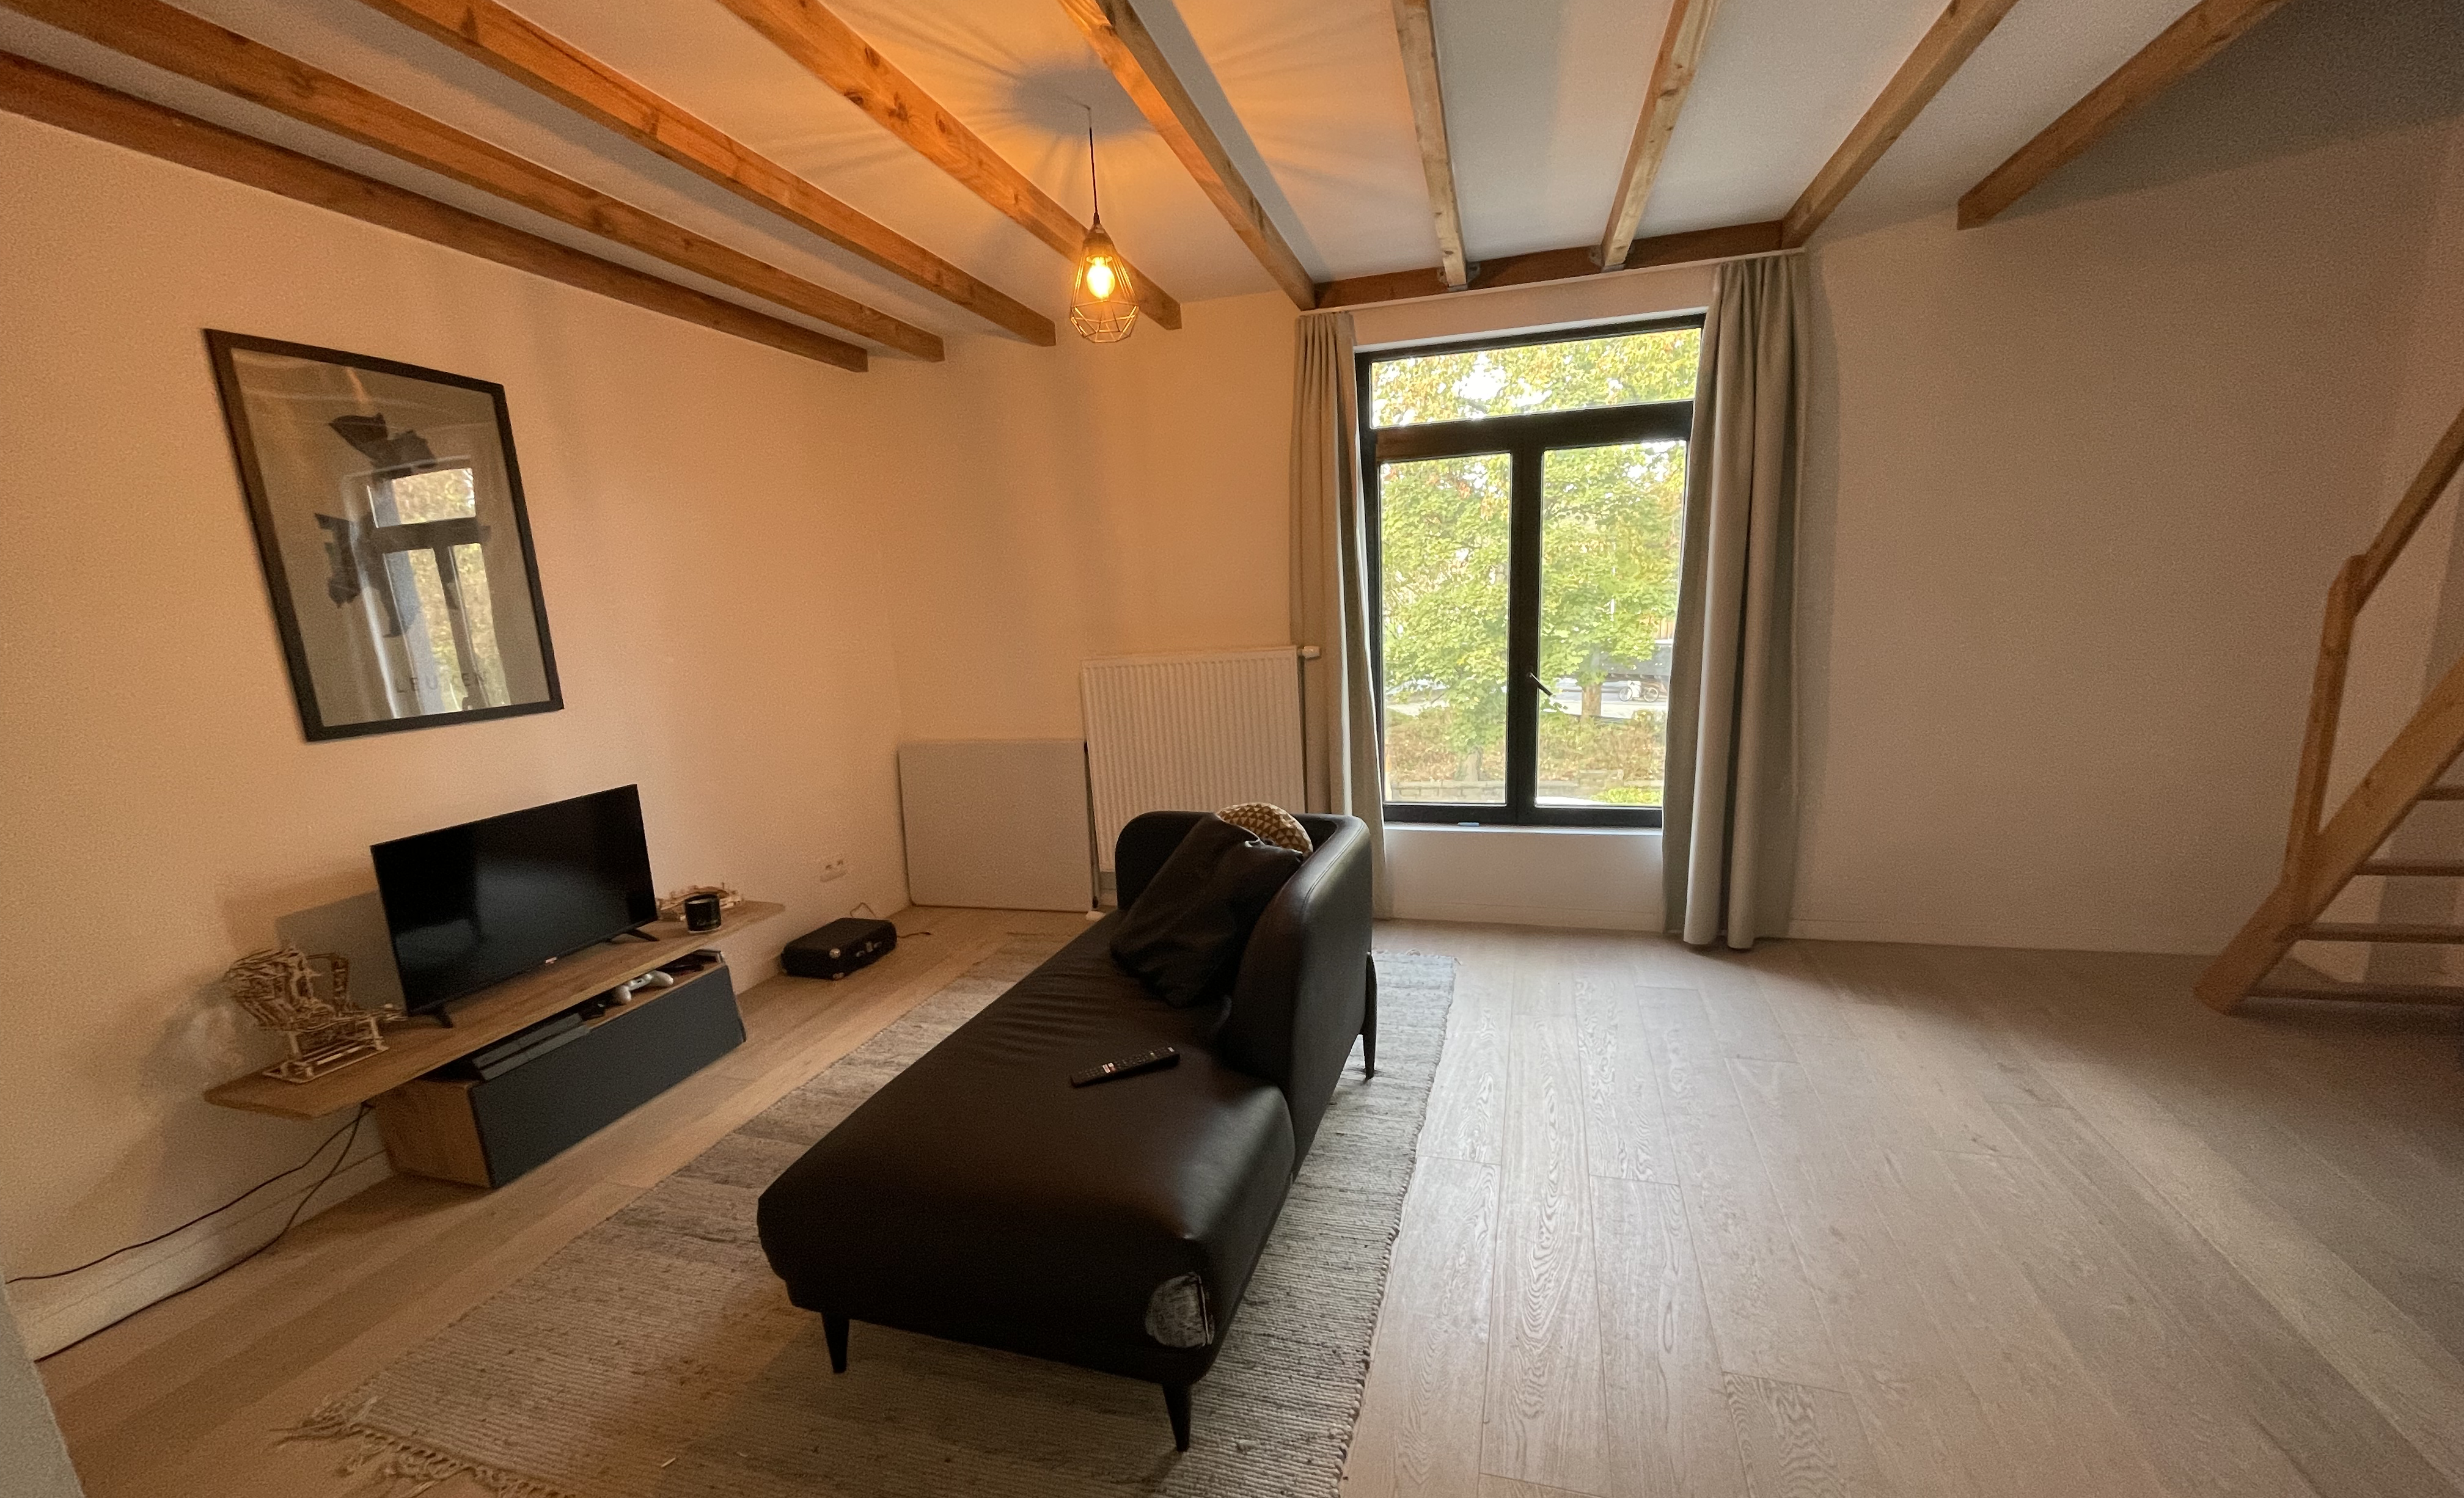
\includegraphics[scale=0.07]{images/apartment.png}
\caption{•}
\label{fig:apartment}
\end{figure}

Here, it can be seen that the apartment is equipped with a large window as well as a single radiator as means of heating. The window faces south, maximizing the solar radiation throughout the day and has an area of 2.1 m$^2$. The radiator has a maximal heating power of 1000 W and is equipped with a Thermostatic Radiator Valve (TRV) to regulate the heating output.

\subsection{Zone Model}
\label{subsec:zone_model}
In order to model the thermal behavior of this apartment, first a model must be developed. This is achieved by lumping the thermal interactions of the apartment as a Resistance-Capacitance (RC) Thermal network. This is a common practice which leads to simplified models and accurate representations of the zone behaviors. Considering that the zone is relatively small in size ($\approx25$ m$^2$), a single zone model was used. Multiple lumped models with increasing number of zones and increasing complexity exist, nevertheless, they were deemed unnecessary. Figure \ref{fig:single_zone} shows the RC-thermal network applied \textbf{CITE MPC IN BUILDINGS PAPER}.

\begin{figure}[H]
\centering
\includegraphics[scale=0.5]{images/single_zone.png}
\caption{•}
\label{fig:single_zone}
\end{figure}

Moreover, an additional heating source $Q_g$ was introduced in order to account for the heat generated by the occupancy of the zone. Table \ref{tab:nomenclature_model} contains descriptions for all the above stated variables alongside their units.

\begin{table}[H]
\centering
\begin{tabular}{c|c|c}
Symbol & Variable & Units \\
\hline
\hline
$T_z$ & Zone average temperature & $K$\\
$T_a$ & Ambient temperature & $K$\\
$R_w$ & Wall thermal resistance & $K/W$\\
$C_z$ & Zone thermal capacitance & $J/K$\\
$gA$ & Window glazing factor $\cdot$ window area & $m^2$\\
$\dot{Q}_g$ & Heat input from occupancy & $W$\\
$\dot{Q}_{sun}$ & Heat input from solar radiation & $W/m^2$\\
$\dot{Q}_h$ & Heat input from radiator & $W$
\end{tabular}
\caption{•}
\label{tab:nomenclature_model}
\end{table}
